%\VignetteIndexEntry{meadq }
%\VignetteKeywords{MEA}
%\VignettePackage{meadq}
%\VignetteEngine{knitr::knitr}
\documentclass{article}\usepackage[]{graphicx}\usepackage[]{color}
%% maxwidth is the original width if it is less than linewidth
%% otherwise use linewidth (to make sure the graphics do not exceed the margin)
\makeatletter
\def\maxwidth{ %
  \ifdim\Gin@nat@width>\linewidth
    \linewidth
  \else
    \Gin@nat@width
  \fi
}
\makeatother

\definecolor{fgcolor}{rgb}{0.345, 0.345, 0.345}
\newcommand{\hlnum}[1]{\textcolor[rgb]{0.686,0.059,0.569}{#1}}%
\newcommand{\hlstr}[1]{\textcolor[rgb]{0.192,0.494,0.8}{#1}}%
\newcommand{\hlcom}[1]{\textcolor[rgb]{0.678,0.584,0.686}{\textit{#1}}}%
\newcommand{\hlopt}[1]{\textcolor[rgb]{0,0,0}{#1}}%
\newcommand{\hlstd}[1]{\textcolor[rgb]{0.345,0.345,0.345}{#1}}%
\newcommand{\hlkwa}[1]{\textcolor[rgb]{0.161,0.373,0.58}{\textbf{#1}}}%
\newcommand{\hlkwb}[1]{\textcolor[rgb]{0.69,0.353,0.396}{#1}}%
\newcommand{\hlkwc}[1]{\textcolor[rgb]{0.333,0.667,0.333}{#1}}%
\newcommand{\hlkwd}[1]{\textcolor[rgb]{0.737,0.353,0.396}{\textbf{#1}}}%

\usepackage{framed}
\makeatletter
\newenvironment{kframe}{%
 \def\at@end@of@kframe{}%
 \ifinner\ifhmode%
  \def\at@end@of@kframe{\end{minipage}}%
  \begin{minipage}{\columnwidth}%
 \fi\fi%
 \def\FrameCommand##1{\hskip\@totalleftmargin \hskip-\fboxsep
 \colorbox{shadecolor}{##1}\hskip-\fboxsep
     % There is no \\@totalrightmargin, so:
     \hskip-\linewidth \hskip-\@totalleftmargin \hskip\columnwidth}%
 \MakeFramed {\advance\hsize-\width
   \@totalleftmargin\z@ \linewidth\hsize
   \@setminipage}}%
 {\par\unskip\endMakeFramed%
 \at@end@of@kframe}
\makeatother

\definecolor{shadecolor}{rgb}{.97, .97, .97}
\definecolor{messagecolor}{rgb}{0, 0, 0}
\definecolor{warningcolor}{rgb}{1, 0, 1}
\definecolor{errorcolor}{rgb}{1, 0, 0}
\newenvironment{knitrout}{}{} % an empty environment to be redefined in TeX

\usepackage{alltt}
\usepackage{mathpazo}
\renewcommand{\sfdefault}{lmss}
\renewcommand{\ttdefault}{lmtt}
\usepackage[T1]{fontenc}
\usepackage[a4paper,left=2cm,right=4cm,top=2cm,bottom=2cm]{geometry}
\usepackage{setspace}
\usepackage{listings}
\usepackage{verbatim}

\usepackage{xspace,amsmath}
\newcommand{\um}{\ensuremath{\mu \text{m}}\xspace}
\usepackage{url}
\usepackage[authoryear]{natbib}
\newcommand{\dynamic}{(Dynamic)}
\newcommand{\static}{(Static)}
\newcommand{\hdfgroup}[1]{\texttt{#1}}
\IfFileExists{upquote.sty}{\usepackage{upquote}}{}


\begin{document}

\onehalfspacing
\title{meadq package: from A to Z}

\author{Diana Hall}
\date{\today}

\maketitle

\section*{Introduction}

This is an introduction to the abilities of the meadq package
for analysis of multielectrode array data.  The program is specifically suited to analyze data from the 12 \& 48 well MEA plates, such as those from Axion Biosystems.  It is not a comprehensive guide, but simply gives examples of what can be done with the package.
The package contains some example data sets which are used here to
demonstrate various routines. 

% * is used to remove the default numbering of sections
\section*{Installation}
To install this package, a binary source code may be used or github may be used for latest version. Package sources via the URL \url{http://github.com/dianaransomhall/meadq}.and then view this introductory vignette

\subsection*{Installation using source}
\begin{knitrout}
\definecolor{shadecolor}{rgb}{0.969, 0.969, 0.969}\color{fgcolor}\begin{kframe}
\begin{alltt}
\hlstd{tarfile.path} \hlkwb{=} \hlstr{"F:/R/Rpackage_meadq/meadq_1.0.1.tar.gz"}
\hlkwd{install.packages}\hlstd{(}\hlkwc{pkgs} \hlstd{= tarfile.path,} \hlkwc{type} \hlstd{=} \hlstr{"source"}\hlstd{,} \hlkwc{repos} \hlstd{=} \hlkwa{NULL}\hlstd{)}
\hlkwd{vignette}\hlstd{(}\hlstr{"meadq-intro"}\hlstd{,} \hlkwc{package} \hlstd{=} \hlstr{"meadq"}\hlstd{)}
\end{alltt}
\end{kframe}
\end{knitrout}


\subsection*{Installation using github }
Alternatively, most recent version meadq may be downloaded from github. ``devtools'' R-package will need to be installed to enable the install\textunderscore github functionality. 
\begin{knitrout}
\definecolor{shadecolor}{rgb}{0.969, 0.969, 0.969}\color{fgcolor}\begin{kframe}
\begin{alltt}
\hlkwd{install.package}\hlstd{(}\hlstr{"devtools"}\hlstd{)}  \hlcom{# note: need R v.>=3.1.0}
\hlcom{# to install devtools, use CRAN}
\hlkwd{require}\hlstd{(devtools)}
\hlkwd{install_github}\hlstd{(}\hlstr{"dianaransomhall/meadq"}\hlstd{)}
\end{alltt}
\end{kframe}
\end{knitrout}



\section{R software reference}
For those new to R, the free software may be downloaded from \url{http://www.cran.r-project.org}.  A highly user-friendly interface may be downloaded here \url{http://www.rstudio.com} with a guide here \url{http://www.dss.princeton.edu/training/RStudio101.pdf}.  A beginners guide to R is available here \url{http://www.cran.r-project.org/doc/contrib/Paradis-rdebuts_en.pdf} and inevitable trouble shooting is best done by googling, as web documentation on R abounds.

\subsection*{Vignette}
To view the introductory vingette:
\begin{knitrout}
\definecolor{shadecolor}{rgb}{0.969, 0.969, 0.969}\color{fgcolor}\begin{kframe}
\begin{alltt}
\hlkwd{vignette}\hlstd{(}\hlstr{"meadq-intro"}\hlstd{,} \hlkwc{package} \hlstd{=} \hlstr{"meadq"}\hlstd{)}
\end{alltt}
\end{kframe}
\end{knitrout}


\subsection*{Setup}
This file is a vignette, written in R, as a reproducible research document.
\begin{knitrout}
\definecolor{shadecolor}{rgb}{0.969, 0.969, 0.969}\color{fgcolor}\begin{kframe}
\begin{alltt}
\hlkwd{require}\hlstd{(sjemea)}
\hlkwd{require}\hlstd{(meadq)}
\hlkwd{require}\hlstd{(knitr)}
\hlstd{opts_chunk}\hlopt{$}\hlkwd{set}\hlstd{(}\hlkwc{cache} \hlstd{=} \hlnum{TRUE}\hlstd{)}
\hlstd{opts_chunk}\hlopt{$}\hlkwd{set}\hlstd{(}\hlkwc{dev} \hlstd{=} \hlstr{"pdf"}\hlstd{)}
\end{alltt}
\end{kframe}
\end{knitrout}


\subsection*{Help pages}
A list of help pages associated with the package is given by:
\begin{knitrout}
\definecolor{shadecolor}{rgb}{0.969, 0.969, 0.969}\color{fgcolor}\begin{kframe}
\begin{alltt}
\hlkwd{help}\hlstd{(}\hlkwc{package} \hlstd{=} \hlstr{"meadq"}\hlstd{)}
\end{alltt}
\end{kframe}
\end{knitrout}





\section*{File naming conventions and experiment log file } 
File names help store meta-data about file as well as provide a unique identifying used in the link to the experiment log file.  The experiment log file serves as more in depth documentation of what was done in experment.  Together the log file and the file name provide redundancy in experimental protocol useful as a check and also make data sets readily usable for those unfamiliar with data.

\subsection*{File naming conventions}
Aspects of the file naming conventions must be followed in order that the code executes without error. Those aspects which much be followed are that the first 4 chunks must be seperated by ``\textunderscore '' and must give meta-data that matches with the experimental log file .csv file. This is necessary for meadq to match the input file to experimental meta-data in the log file and combine them in the resulting hdf5 file. 
\\*Let's use the example file provdied within the package subdirectory``extdata'': 

\begin{description}
\item[spike train text file]
ON\textunderscore 20140205\textunderscore MW1007-26\textunderscore DIV07\textunderscore 001.mapTimestamps 
\item[log file] Experiment\textunderscore LogFileExample.csv
\end{description}


\begin{description}

\item[Project] ``ON'' codes the project or group of experiments: ``ON'' for ontogeny. 
\begin{description}
\item[position in file name] immediately preceeding the first `\textunderscore '
\item[format] The project desination may be of any length or capitalization but needs to begin with a letter.
\item[designation in log file] The corresponding column in the log file must be entitled ``Project''. The contents of the ``Project'' column in the log file and the project designation in file name must be identical.
\end{description}


\item[Experiment Date] ``20140205'' denotes the date of the plating of the neurons, February 5, 2014. 
\begin{description}
\item[position in file name] immediate following the first `\textunderscore '
\item[format] YYYYMMDD 
\item[designation in log file] The corresponding column in the log file must be entitled ``Experiment Date''. The contents of the ``Experiment Date'' column in log file must be identical to the Experiment Date designation in file name.
\end{description}


\item[Plate SN ]  ``MW1007-26'' is the serial number (SN) of the plate used in the recording.  
\begin{description}
\item[position in file name] The serial number always follows the second `\textunderscore '.
\item[format] any format alpha or numeric, so long as serial number contains no  \textunderscore
\item[designation in log file] The corresponding column in the log file must be entitled ``Plate SN''. The contents of column entitled ``Plate SN'' in the log file must be identical to the plate serial number designation in the file name.
\end{description}

\item[DIV] ``DIV07'' denotes the 7th day in vitro (DIV) of the plated cells.
\begin{description}
\item[position in file name] After the 3rd ` \textunderscore '.
\item[format]  ``DIV07'', ``DIV7'', ``07'', ``7'' are all permissible so long as a exact match is made to log file.
\item[designation in log file] The DIV column in the log file must be entitled ``DIV''. The contents of the ``DIV'' column in the log file and the DIV designation in the file name must be identical.
\end{description}

\item[Users Choice] Any other naming conventions may be added to end of file name. Example data has `001' to indicate sequential order of recording should more than one be made with same meta-data.  Other examples may include indication of `pre' or  `post'  should there be pre and pose dose recordings.

\end{description}




\subsection*{Experiment log file conventions}
Experiment log file must be a .csv (comma seperated value) file that contain the names and information listed below.  See  ``Experiment\textunderscore LogFileExample.csv'' located in the ``extdata'' subdirectory of package for an example.

Column names in log file must match verbatim to list below (case sensitive):
\begin{description}
\item[Project] \mbox{}\\
\begin{description}
\item[format] Must match file name.  See ``Project'' in above subsection.
\end{description}

\item[Experiment Date] \mbox{}\\
\begin{description}
\item[format] Must match file name. See ``Experiment Date'' in above subsection.  
\end{description}

\item[Plate SN] \mbox{}\\
\begin{description}
\item[format] Must match file name. See ``Plate SN'' in above subsection.  
\end{description}


\item[DIV] \mbox{}\\
\begin{description}
\item[format] Must correspond to file name. See ``DIV'' in above subsection. 
\end{description}


\item[Well] \mbox{}\\
\begin{description}
\item[format] one row in log file for each well; must be a capital letter preceeded by a number e.g. "A1"or "F3" 
\end{description}

\item[Treatment] \mbox{}\\
\begin{description}
\item[format] any character string without spaces is permissible.
\end{description}

\item[Size] \mbox{}\\
\begin{description}
\item[format] give any size data about anything or list NA in column if no size specification exist 
\end{description}

\item[Dose] \mbox{}\\
\begin{description}
\item[format] dose of treatment. Any rational, or integer number is permissible 
\end{description}

\item[Units] \mbox{}\\
\begin{description}
\item[format] any-alpha numeric unit specification is permissible 
\end{description}

\end{description}






\section*{Creating HDF5 Files}
Converting data into HDF5 file format is beneficial for many reasons. Firstly, converting the recorded data from a proprietary or otherwise restrictive file type into a universal file type, such as HDF5, facilitates data sharing and provides flexibility in analysis software choice.  Secondly, the ``program on standards for datasharing'' by the International Neuroinformatics Coordinating Facility \url{ http://www.datasharing.incf.ord/ep/HDF5_data_standard} has recommended the HDF5 format. Finally, HDF5 files are designed to store meta-data and data seperately for maximum efficiency. For more information of the HDF5 format see \url{http://www.hdfgroup.org/HDF5/doc/H5.into.html}.
 Code is provided to convert axion alpha map files (.map extension) to text files and finally to HDF5 (.h5 extention) format files and in the process store meta-data inside recording file. The intermediate step of converting alpha map files to text files is necessary since alpha map files are in binary and may only be decoded by a third party software such as NeuroExplorer \citep{neuroexplorer}.

\subsection{create text files from alpha map files} \mbox{}\\
NeuroExplorer has a scripting language that may be used to batch create text files (.mapTimestamps extension) of spike trains from apha map files.  meadq needs text spike trains to use the ``.mapTimestamps'' file extension.  For information regarding script language see manual
here \url{http://www.neuroexplorer.com/downloads/Nex3Manual.pdf}.  A neuroExplorer script entitled ``Export\textunderscore timestamps\textunderscore from\textunderscore map\textunderscore files\textunderscore meadqExample.nsc'' is provided in the ``extdata'' subdirectory of
meadq folder. 

\subsection*{Execution}
\begin{description}
\item[interactive session] The script may be executed by initiating an interactive session of NeuroExplorer, opening the script and clicking the green play button.  A dialogue box will appear in the NeuroExplorer main page prompting for user to enter directory containing .map files to be converted.  Enter the file path where the .map files are located (make sure to keep the ``.\text{*}map'') and press ok.  The script outputs the .mapTimestamp files in the same folder as the .map files.  Try running the script on the example .map file provided in the ``extdata'' folder entitled ``ON\textunderscore 20140205\textunderscore MW1007-26\textunderscore DIV05\textunderscore 001.map ''

\end{description}


``Export\textunderscore timestamps\textunderscore from\textunderscore map\textunderscore files\textunderscore meadqExample.nsc''

\begin{verbatim}
doc = 0
filefilter ="C:/Users/dhall05/Desktop/*.map"
res = Dialog(doc, filefilter, "File Filter:", "string" )
% create save folder
position1 = Find(filefilter, "*" )
save_folder = Left( filefilter, position1-1)

Trace(save_folder, " timestamps have been saved in a text file")
n= GetFileCount(filefilter)

Trace(n, "files")
for i=1 to n
name = GetFileName(i)
doc = OpenDocument (name)
doc_title=GetDocTitle(doc)
save_path= save_folder + doc_title + ".mapTimestamps"

stampslabel = GetDocPath(doc) + "Timestamps"
if doc > 0
SaveAsTextFile(doc, save_path)
Trace(name, "timestamps have been saved in a text file")
CloseDocument(doc)
end
end
\end{verbatim}

\subsection{create HDF5 files from text files}


\begin{knitrout}
\definecolor{shadecolor}{rgb}{0.969, 0.969, 0.969}\color{fgcolor}\begin{kframe}
\begin{alltt}
\hlcom{## }
\hlstd{data.file} \hlkwb{<-} \hlkwd{system.file}\hlstd{(}\hlstr{"extdata"}\hlstd{,} \hlstr{"ON_20140205_MW1007-26_DIV07_001.mapTimestamps"}\hlstd{,}
    \hlkwc{package} \hlstd{=} \hlstr{"meadq"}\hlstd{)}
\hlcom{# user will be promted to navigate to .mapTimestamps files & log file}
\hlkwd{make.axion.map.to.h5.dh}\hlstd{()}
\end{alltt}
\end{kframe}
\end{knitrout}









\section*{Create well summary spreadsheet}
Create two csv files \colon

\begin{description}
\item[ ont\textunderscore data\textunderscore summary\textunderscore AEfilt.csv] computes well summaries for each file using all AE (active electrodes\colon  $\geq 5$ spikes/min ) 
\item[ ont\textunderscore data\textunderscore summary\textunderscore ABEfilt.csv] computes well summaries for each file using all ABE (actively bursting electrodes\colon  $\geq 1$ burst/min)
\end{description}

\begin{knitrout}
\definecolor{shadecolor}{rgb}{0.969, 0.969, 0.969}\color{fgcolor}\begin{kframe}
\begin{alltt}
\hlstd{data.file1} \hlkwb{<-} \hlkwd{system.file}\hlstd{(}\hlstr{"extdata"}\hlstd{,} \hlstr{"ON_20140205_MW1007-26_DIV05_001.h5"}\hlstd{,} \hlkwc{package} \hlstd{=} \hlstr{"meadq"}\hlstd{)}
\hlstd{data.file2} \hlkwb{<-} \hlkwd{system.file}\hlstd{(}\hlstr{"extdata"}\hlstd{,} \hlstr{"ON_20140205_MW1007-26_DIV07_001.h5"}\hlstd{,} \hlkwc{package} \hlstd{=} \hlstr{"meadq"}\hlstd{)}
\hlstd{data.file3} \hlkwb{<-} \hlkwd{system.file}\hlstd{(}\hlstr{"extdata"}\hlstd{,} \hlstr{"ON_20140205_MW1007-26_DIV09_001.h5"}\hlstd{,} \hlkwc{package} \hlstd{=} \hlstr{"meadq"}\hlstd{)}
\hlstd{h5Files} \hlkwb{=} \hlkwd{c}\hlstd{(data.file1, data.file2, data.file3)}
\hlstd{param.file} \hlkwb{<<-} \hlkwd{system.file}\hlstd{(}\hlstr{"data"}\hlstd{,} \hlstr{"chgv_parameters.rda"}\hlstd{,} \hlkwc{package} \hlstd{=} \hlstr{"meadq"}\hlstd{)}

\hlkwd{create_ont_csv}\hlstd{(}\hlkwc{h5Files} \hlstd{= h5Files,} \hlkwc{save.rdata} \hlstd{=} \hlnum{TRUE}\hlstd{,} \hlkwc{param.file} \hlstd{= param.file)}
\end{alltt}
\end{kframe}
\end{knitrout}



In the process of making the well summary, a rdata (R's native data type) has been created in the same directory where the .h5 files are located, as save.rdata argument was set to TRUE.  Rdata or .rda extention is easily loadable by R using the following commands:
\begin{knitrout}
\definecolor{shadecolor}{rgb}{0.969, 0.969, 0.969}\color{fgcolor}\begin{kframe}
\begin{alltt}
\hlstd{data.file} \hlkwb{<-} \hlkwd{system.file}\hlstd{(}\hlstr{"data"}\hlstd{,} \hlstr{"example_ont_data.rda"}\hlstd{,} \hlkwc{package} \hlstd{=} \hlstr{"meadq"}\hlstd{)}
\hlkwd{load}\hlstd{(data.file)}
\end{alltt}
\end{kframe}
\end{knitrout}






\section*{What is the ``s[[i]]'' object?}

A convention of the program is that all data referring to a recording
is stored within an object of class \texttt{mm.s}, which is actually a
list.  So, when new data/results are collected for a recording, I tend
to add the new information into that object (e.g. see how burst
analysis results are stored).

The most important items in the list are:
\begin{description}
\item[NCells] The number of units in the recording.
\item[rec.time] The start and end time of the recording.
\item[spikes] A list of vectors.  Element $i$ of the list is the
  vector of spike trains for unit $i$.  Each spike train is ordered, smallest first.
\item[nspikes] A vector.  $nspikes[i]$ is the number of spikes in
  train i.
\item[layout] Information regarding the spatial layout of the units.
\end{description}











\section*{Burst analysis}

There are several routines for burst analysis. The most common is implemented:

\begin{enumerate}
\item Max Interval method, as described by Neuroexplorer \citep{neuroexplorer}

\end{enumerate}

\begin{knitrout}
\definecolor{shadecolor}{rgb}{0.969, 0.969, 0.969}\color{fgcolor}\begin{kframe}
\begin{alltt}
\hlkwd{data}\hlstd{(}\hlstr{"example_ont_data"}\hlstd{)}
\end{alltt}
\end{kframe}
\end{knitrout}


So, for example, for electrode 2, we see the following bursts (just
taking the head as there are many of them.  We can also easily plot
the number of bursts on each electrode.

\begin{knitrout}
\definecolor{shadecolor}{rgb}{0.969, 0.969, 0.969}\color{fgcolor}\begin{kframe}
\begin{alltt}
\hlstd{s[[}\hlnum{3}\hlstd{]]}\hlopt{$}\hlstd{channels[[}\hlnum{2}\hlstd{]]}
\end{alltt}
\begin{verbatim}
## [1] "A1_12"
\end{verbatim}
\begin{alltt}
\hlkwd{head}\hlstd{(s[[}\hlnum{3}\hlstd{]]}\hlopt{$}\hlstd{allb[[}\hlnum{2}\hlstd{]])}
\end{alltt}
\begin{verbatim}
##      beg end    IBI len   durn mean.isis SI
## [1,]   6  22     NA  17 0.3415   0.02135  1
## [2,]  27  31  4.905   5 0.2251   0.05628  1
## [3,]  36  42  2.818   7 0.8008   0.13347  1
## [4,]  55  76  9.969  22 0.6484   0.03088  1
## [5,]  98 103 21.426   6 0.9942   0.19885  1
## [6,] 129 134 14.458   6 0.6998   0.13997  1
\end{verbatim}
\begin{alltt}
\hlstd{nbursts} \hlkwb{<-} \hlkwd{sapply}\hlstd{(s[[}\hlnum{3}\hlstd{]]}\hlopt{$}\hlstd{allb, nrow)}
\hlkwd{plot}\hlstd{(nbursts,} \hlkwc{xlab} \hlstd{=} \hlstr{"Electrode number"}\hlstd{,} \hlkwc{ylab} \hlstd{=} \hlstr{"Number of bursts"}\hlstd{,} \hlkwc{bty} \hlstd{=} \hlstr{"n"}\hlstd{,}
    \hlkwc{las} \hlstd{=} \hlnum{1}\hlstd{)}
\end{alltt}
\end{kframe}
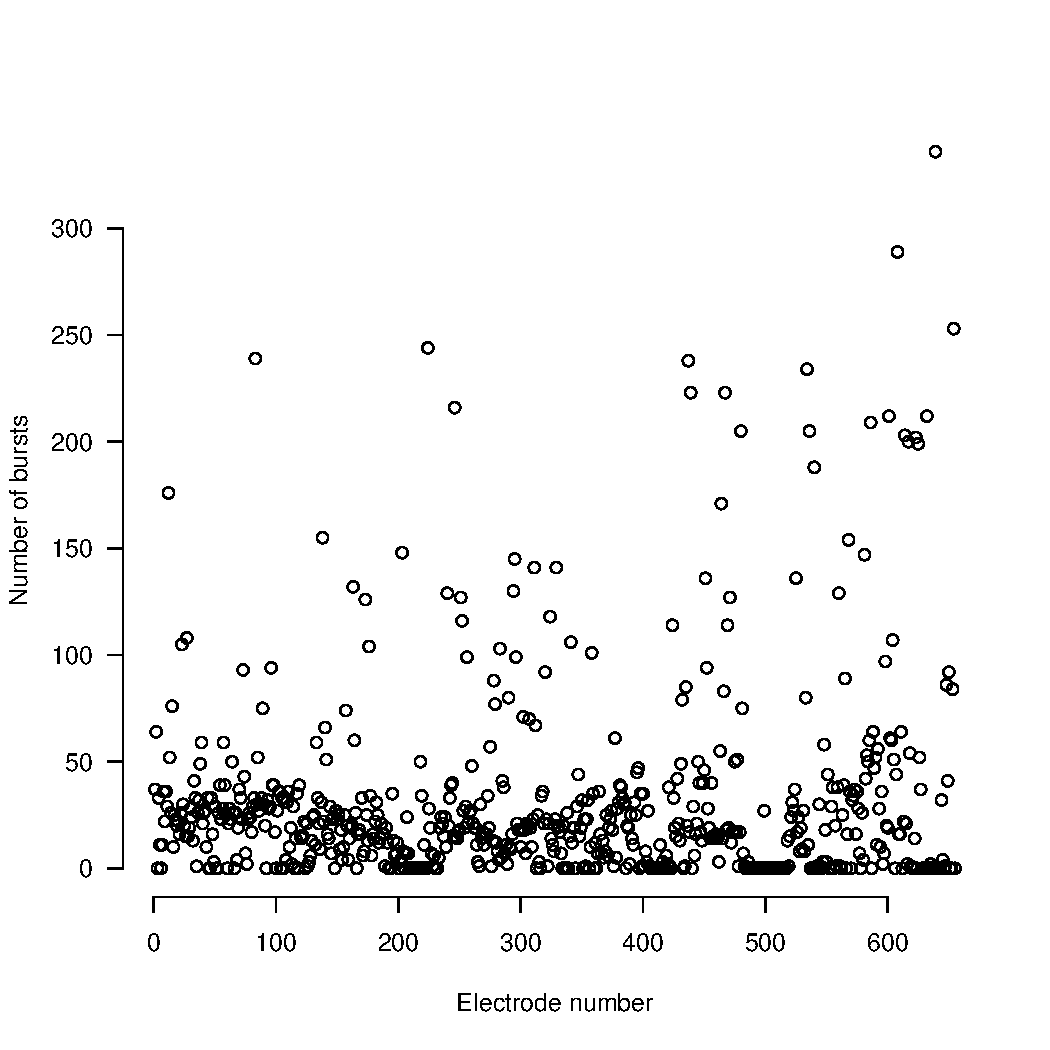
\includegraphics[width=\maxwidth]{figure/show-burst-info} 

\end{knitrout}



Once bursts are computed the resulting burst information can be
visualized on a raster assuming that the burst information is stored
in the \verb+s$allb+ component of the object.  Here we ask to see the
burst information for twenty seconds of data from just the first five trains.

\begin{knitrout}
\definecolor{shadecolor}{rgb}{0.969, 0.969, 0.969}\color{fgcolor}\begin{kframe}
\begin{alltt}
\hlkwd{plot}\hlstd{(s[[}\hlnum{2}\hlstd{]],} \hlkwc{beg} \hlstd{=} \hlnum{200}\hlstd{,} \hlkwc{end} \hlstd{=} \hlnum{250}\hlstd{,} \hlkwc{show.bursts} \hlstd{=} \hlnum{TRUE}\hlstd{,} \hlkwc{whichcells} \hlstd{=} \hlnum{1}\hlopt{:}\hlnum{5}\hlstd{)}
\end{alltt}
\end{kframe}
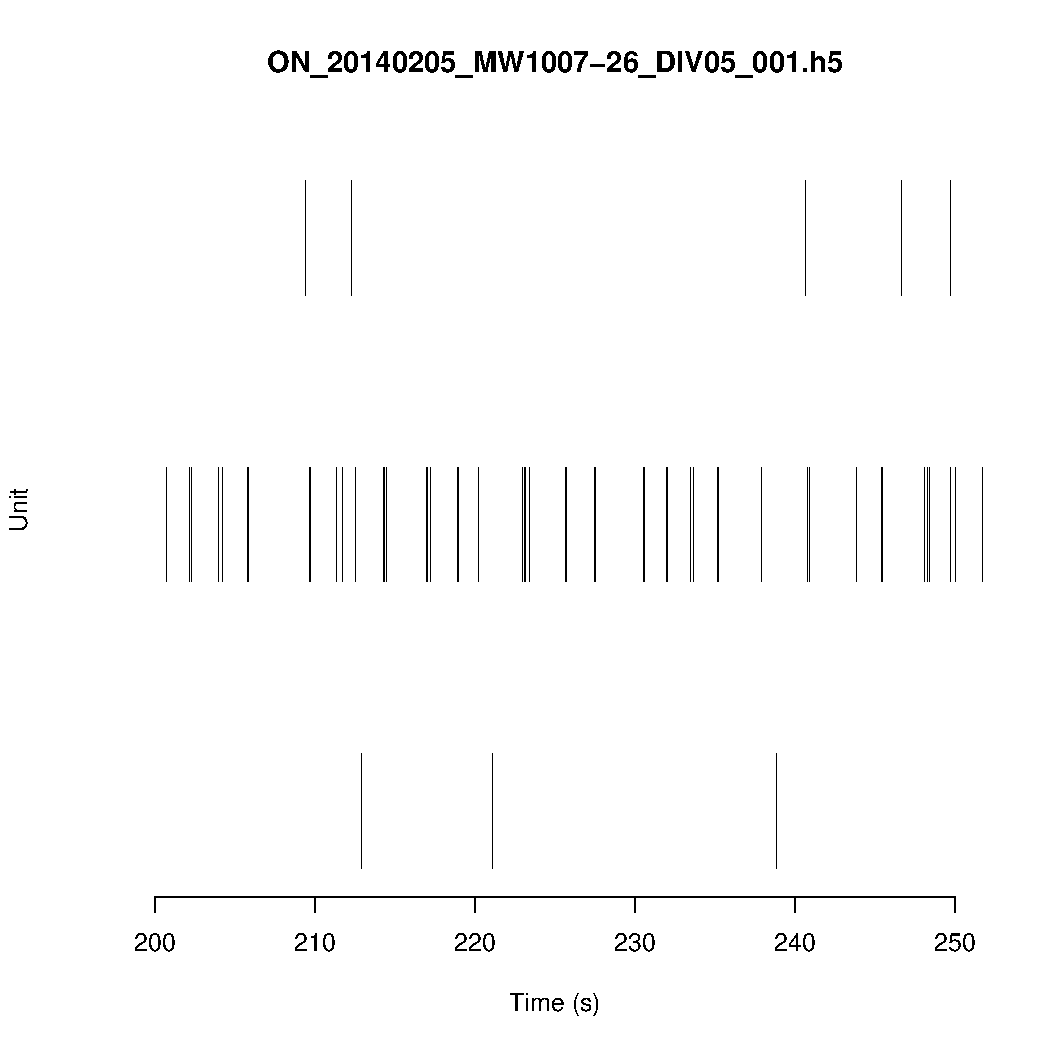
\includegraphics[width=\maxwidth]{figure/burst-raster} 

\end{knitrout}


Bursts are indicated with a red horizontal line, and the blue number
indicates the number of spikes in the burst.


Note: a Hidden-Markov Model (HMM) for burst analysis in R \citep{Tokdar2010}
is available in the following package:
\url{http://www.stat.duke.edu/~st118/Software/}.

can be used within this package, but in principle (computation time
aside as I expect an HMM to be slow) there should be no issue.  There
is also a generic ``bursts'' package:
\url{http://cran.r-project.org/web/packages/bursts/bursts.pdf}.



\section*{Plate Summary Graphics}

Get summary graphics of one of multiple files.

\begin{knitrout}
\definecolor{shadecolor}{rgb}{0.969, 0.969, 0.969}\color{fgcolor}\begin{kframe}
\begin{alltt}
\hlstd{h5Files} \hlkwb{=} \hlkwd{system.file}\hlstd{(}\hlstr{"data"}\hlstd{,} \hlstr{"example_ont_data.rda"}\hlstd{,} \hlkwc{package} \hlstd{=} \hlstr{"meadq"}\hlstd{)}
\hlstd{param.file} \hlkwb{=} \hlkwd{system.file}\hlstd{(}\hlstr{"data"}\hlstd{,} \hlstr{"chgv_parameters.rda"}\hlstd{,} \hlkwc{package} \hlstd{=} \hlstr{"meadq"}\hlstd{)}

\hlkwd{burst_table_Plots}\hlstd{(}\hlkwc{param.file} \hlstd{= param.file,} \hlkwc{h5Files} \hlstd{= h5Files)}
\end{alltt}
\end{kframe}
\end{knitrout}






\section*{PCA: Principle components analysis}

PCA is a useful technique in the MEA data framework. Many variables or ``features'' may be derived from a spike train without knowing which among these best capture the inforation in data.  PCA takes high-dimensional data, so called for the many variables such as mean firing rate, inter burst interval, etc. comprising the data, and identifies combinations of those variables, or PC dimensions, that are responsible for the greatest percentage of variation.  In this manner, a few PC dimensions describe a large percentage of variation in the data thereby reducing the number of variables, or dimensionality, of the data.

\begin{knitrout}
\definecolor{shadecolor}{rgb}{0.969, 0.969, 0.969}\color{fgcolor}\begin{kframe}
\begin{alltt}
filename.data = 
trt.params.wanted = 
output.folder = 
ctr.params.wanted = 
vars.wanted = 

\end{alltt}
\end{kframe}
\end{knitrout}














\section*{Network spikes: sjemea pacakge }

Network spikes are periodic elevations in activity across the whole
array \citep{Eytan2006}.  The following example shows how they are computed.
In the resulting graph, the population ``firing rate'' (the number of
active electrodes here) is shown on the y axis, time (in seconds) on
the x axis.  The horizontal red line is a threshold set for the
minimum number of active electrodes to determine a ``network spike''.
The blue dots are the peak of each network spikes.

The mean network spike is also shown, averaged across all the network
spikes in the recording.

\begin{knitrout}
\definecolor{shadecolor}{rgb}{0.969, 0.969, 0.969}\color{fgcolor}\begin{kframe}
\begin{alltt}
\hlkwd{example}\hlstd{(compute.ns)}
\end{alltt}
\end{kframe}
\end{knitrout}


\section*{Correlation index: sjemea package}

The correlation index plot was devised by \citet{Wong1993} as a method to
estimate how correlation between any pair of neurons on the array
depends (if at all) upon the distance separating the pair.  For
retinal waves, the correlation index usually has an
exponentially-decaying profile.  For other recordings,
(e.g. hippocampal cultures), the profile tends to be flatter.

\begin{knitrout}
\definecolor{shadecolor}{rgb}{0.969, 0.969, 0.969}\color{fgcolor}\begin{kframe}
\begin{alltt}
\hlstd{jay.data.file} \hlkwb{<-} \hlkwd{system.file}\hlstd{(}\hlstr{"examples"}\hlstd{,} \hlstr{"P9_CTRL_MY1_1A.txt"}\hlstd{,} \hlkwc{package} \hlstd{=} \hlstr{"sjemea"}\hlstd{)}
\hlstd{jay.s} \hlkwb{<-} \hlkwd{jay.read.spikes}\hlstd{(jay.data.file)}
\hlkwd{plot.corr.index}\hlstd{(jay.s)}
\end{alltt}


{\ttfamily\noindent\color{warningcolor}{\#\# Warning: removing 17 zero entries}}\end{kframe}
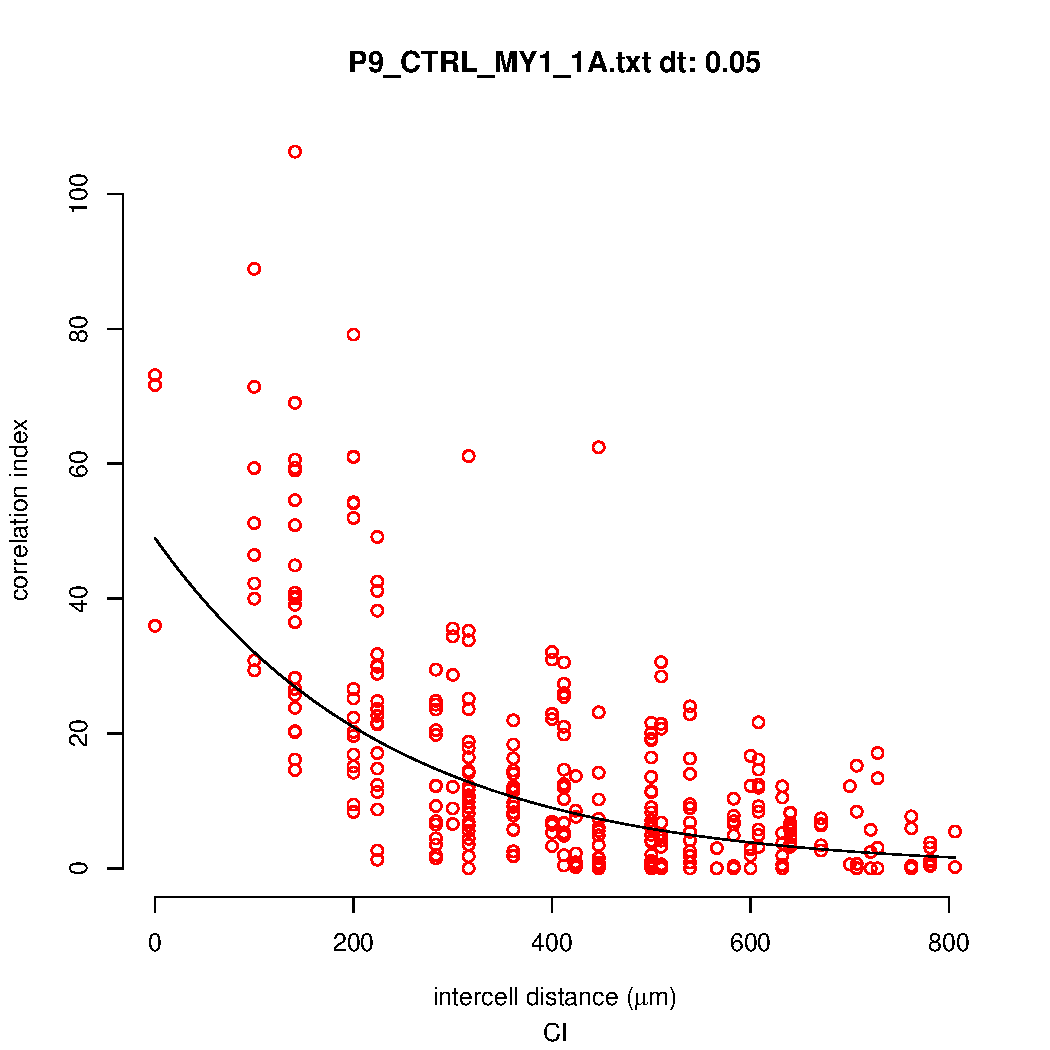
\includegraphics[width=\maxwidth]{figure/correlation-index} 

\end{knitrout}


\subsection*{Correlation analysis: sjemea package }

We propose a new tiling-based measure for measuring the correlation
between pairs of spike trains (ongoing work by Catherine Cutts).  Here
is an example of how to compute a tiling correlation matrix for a
group of spike trains.

\begin{knitrout}
\definecolor{shadecolor}{rgb}{0.969, 0.969, 0.969}\color{fgcolor}\begin{kframe}
\begin{alltt}
\hlstd{data.file} \hlkwb{<-} \hlkwd{system.file}\hlstd{(}\hlstr{"examples"}\hlstd{,} \hlstr{"P9_CTRL_MY1_1A.txt"}\hlstd{,} \hlkwc{package} \hlstd{=} \hlstr{"sjemea"}\hlstd{)}
\hlstd{s} \hlkwb{<-} \hlkwd{jay.read.spikes}\hlstd{(data.file)}
\hlstd{t2} \hlkwb{<-} \hlkwd{tiling.allpairwise}\hlstd{(s)}
\hlkwd{require}\hlstd{(lattice)}
\end{alltt}


{\ttfamily\noindent\itshape\color{messagecolor}{\#\# Loading required package: lattice}}\begin{alltt}
\hlkwd{levelplot}\hlstd{(t2)}
\end{alltt}
\end{kframe}
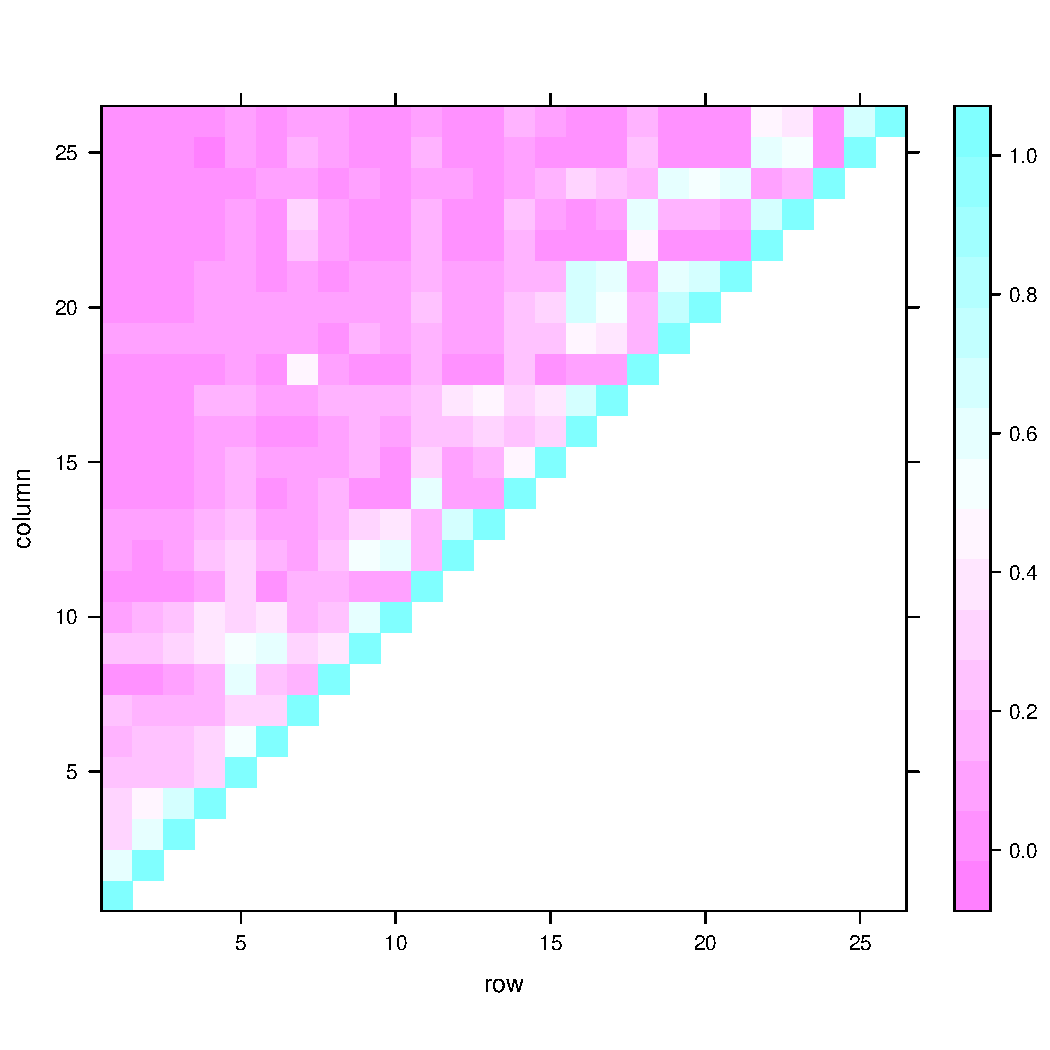
\includegraphics[width=\maxwidth]{figure/tiling-correlation} 

\end{knitrout}




\subsection*{Acknowledgements}
Thanks to Stephen Eglen at DAMTP, Cambridge UK for his help in creating this package by building off of his package ``sjemea'', available \url{http://github.com/sje30/sjemea}.  Thanks to Tim Shafer, US EPA for his help and data.


\bibliographystyle{jneurosci}
\bibliography{sjemea}

\subsection*{Compiling this document}

\begin{knitrout}
\definecolor{shadecolor}{rgb}{0.969, 0.969, 0.969}\color{fgcolor}\begin{kframe}
\begin{alltt}
\hlkwd{require}\hlstd{(knitr)}
\hlkwd{knit2pdf}\hlstd{(}\hlstr{"meadq-intro.Rnw"}\hlstd{)}
\end{alltt}
\end{kframe}
\end{knitrout}





\end{document}
